\documentclass[10pt, xcolor=rgb]{beamer}
\usepackage{graphicx}
\usepackage{soul}
\usepackage{pdfpages}



% choosing the themes
%---------------------------------------------------------------------------------------------
\usetheme{Madrid}
\useinnertheme{default}
\setbeamertemplate{sections/subsections in toc}[sections numbered]

\beamertemplatenavigationsymbolsempty

% redefining the footline with QMUL logo
%----------------------------------------------------------------------------------------------
\setbeamerfont{author in head/foot}{size=\scriptsize}

\makeatletter
\setbeamertemplate{footline}{% override the footline from Madrid
  \leavevmode%
  \hbox{%
  \begin{beamercolorbox}[wd=.333333\paperwidth,ht=8ex,dp=1ex,center]{author in head/foot}%
    \usebeamerfont{author in head/foot}\insertshortauthor \vspace*{1ex}
  \end{beamercolorbox}%
  \begin{beamercolorbox}[wd=.333333\paperwidth,ht=8ex,dp=1ex,center]{title in head/foot}%
   \usebeamerfont{author in head/foot}\insertshorttitle \vspace*{1ex}
  \end{beamercolorbox}%
  \begin{beamercolorbox}[wd=.333333\paperwidth,ht=8ex,dp=1ex,right]{date in head/foot}%
      \raisebox{-0.5mm}{
\includegraphics[height=8ex]{Immagini/Logo_reverse_QMUL}}\hspace*{6ex} \insertframenumber{} \hspace*{2ex} 
  \end{beamercolorbox}}%
  \vskip0pt%
}
\makeatother


%languages and fonts
%------------------------------------------------------------------------------------
\usepackage[utf8]{inputenc}
\usepackage[UKenglish]{babel}
\usepackage[T1]{fontenc}
\usepackage{palatino}


%% math
%%------------------------------------------------------------------------------------
\usepackage{amsfonts, amsmath, amsthm, amssymb, mathrsfs, amscd}		
\usepackage{xfrac}


\usepackage{tikz}
\usetikzlibrary{mindmap}
\usetikzlibrary{chains}
\usetikzlibrary{positioning,calc} 
\tikzset{shifted by/.style={to path={($(\tikztostart)!#1!90:(\tikztotarget)$)
 -- ($(\tikztotarget)!#1!-90:(\tikztostart)$)}}, 
 shifted by/.default=2pt,standard edge/.style={very thick,-latex}, 
 back and forth between/.style args={#1 and #2}{insert path={
  #1 edge[standard edge,-latex,shifted by] #2 #2 edge[standard edge,shifted by] #1}}} 
\usepackage{smartdiagram}
\tikzset{
  treenode/.style = {shape=rectangle, rounded corners, font=\large,
                     draw, align=center,
                     top color=white,
                     bottom color=darkorange!30},
  desc/.style = {shape=rectangle, rounded corners, align=center, bottom color=white},
  root/.style    = {treenode, font=\Large,
                     bottom color=darkpurple!30},
  env/.style      = {treenode},
}


% tables
%--------------
%tables & pictures
%------------------------------------------------------------------------------------
\usepackage{multirow,bigdelim, caption, longtable} % longtable for tables that can fit on multiple pages
\captionsetup[longtable]{position=below} 
\usepackage{booktabs}
\usepackage{graphicx}


 
% named colours
%-------------------------------------------------------------------------------------------
% Primary QMUL palette
\definecolor{bluQM}{RGB}{18, 49, 129}
\definecolor{title}{rgb}{255, 255, 255} 
\definecolor{background}{RGB}{255,255,255}


% Secondary QMUL palette
\definecolor{darkpurple}{RGB}{121, 34, 115}
\definecolor{darkorange}{RGB}{210,092,021}
\definecolor{darkyellow}{RGB}{205, 166, 012}
\definecolor{darkgreen}{RGB}{16, 116, 106}
\definecolor{darkgrey}{RGB}{64,64,64}


% using the colours
%-------------------------------------------------------------------------------------------
\setbeamercolor{title}{fg=title}
\setbeamercolor{subtitle}{fg=title}
\setbeamercolor{frame title}{fg=bluQM}
\setbeamercolor{institute}{fg=darkgray}
\setbeamercolor{author}{fg=darkgray}
\setbeamercolor{structure}{fg=bluQM}
\setbeamercolor{item}{fg=darkgreen} % color of bullets
\setbeamercolor{subitem}{fg=darkorange}
\setbeamercolor{itemize/enumerate subbody}{fg=darkgreen}


\setbeamercolor{block title}{use=bluQM,fg=title,bg=darkgreen}
\setbeamercolor{block body}{use=structure, fg=black,bg=bluQM!10}

\setbeamercolor{frame number in foot}{fg=white!50!bluQM}

\setbeamercolor{alerted text}{fg=darkgreen}

\setbeamercolor{block title example}{use=example text,fg=white,bg=darkgreen!50!white}
\setbeamercolor{block body example}{fg=black,bg=bluQM!10}

\setbeamercolor{block title alerted}{use=alerted text,fg=white,bg=darkpurple}
\setbeamercolor{block body alerted}{fg=black,bg=darkorange!20}


\setbeamercolor{titlelike}{parent=palette primary,fg=bluQM}
\setbeamercolor{frametitle}{bg=bluQM,fg=white}
% \setbeamercolor{frametitle right}{bg=gray!60!white}
% 
\setbeamercolor*{separation line}{}
\setbeamercolor*{fine separation line}{}


% QMUL's logos
% ---------------------------------------------------------------------------------------------

\titlegraphic{
\includegraphics[width=4cm]{Immagini/LogoQM}}
%\logo{
\includegraphics[width=.2\textwidth]{Immagini/LogoQM}}


% Title info
%---------------------------------------------------------------------------------------------
\title{STAT 5 tutorial}
\subtitle{}
\author{Celeste Damiani}
\institute{}
\date{\today}

\begin{document}
{
\setbeamercolor{background canvas}{bg=}
\includepdf[pages=1]{QM-presentation-template.pdf}
}


%% title slide
%\frame[plain]
%{
%  \titlepage
% }
%


\frame{
   \frametitle{This session}
   \tableofcontents
}


\section{Review of case-control and cohort studies designs}
\frame{
	\frametitle{Observational studies}
\begin{columns}
	\begin{column}{0.45\textwidth}
	\begin{block}{Observational studies}
	\begin{itemize}
	\item The investigator simply observers...
	\item ...but has control over:
	\begin{itemize}
		\item\textbf{choice of subjects}
		\item \textbf{follow subjects prospectively or retrospectively}
		\item \textbf{size of the sample}
	\end{itemize}
	
	\end{itemize}
	\end{block}
	\end{column}
	\begin{column}{0.45\textwidth}
		\begin{block}{Randomised controlled trials}
		Examine the relative efficacy of treatments or \textbf{interventions} in human subjects.
	
	\end{block}
	\end{column}
\end{columns} 
}


\frame{
	\frametitle{Case-control and cohort studies}
\begin{center}
\large{\ul{Cohort study}}
\end{center}
\begin{center}
\scalebox{.5}{
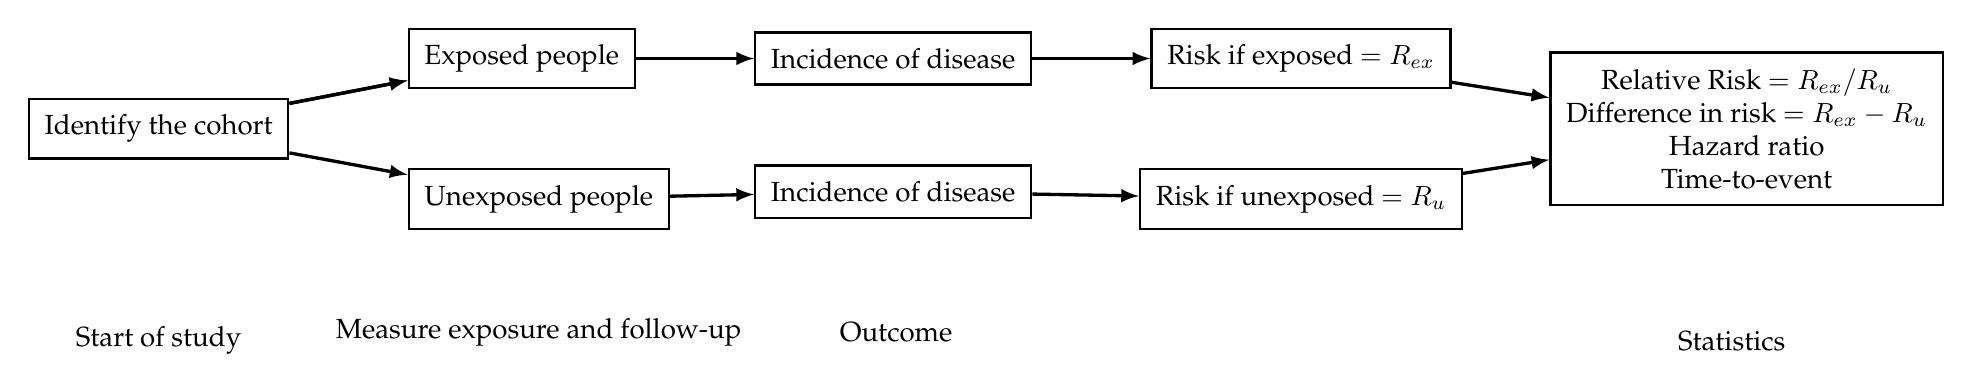
\begin{tikzpicture}[boot/.style={draw,thick,align=center, inner sep=2mm}]
\node[boot=20] (CH) {Identify the cohort};
\node[above right=0.5cm and 1.5cm of CH.east,boot=20] (EP) {Exposed people};
\node[below right=0.5cm and 1.5cm of CH.east,boot=20] (UP) {Unexposed people};
\node[right=1.5cm of EP,boot=20] (ID1) {Incidence of disease};
\node[right=1.5cm of UP, below=1cm of ID1, boot=20] (ID2) {Incidence of disease};
\node[right=1.5cm of ID1,boot=20] (RE) {Risk if exposed $= R_{ex}$};
\node[right=1.5cm of ID2, below=1cm of RE, boot=20] (RU) {Risk if unexposed $= R_{u}$};
\node[right=16cm of CH,boot=20] (STAT) {Relative Risk $= R_{ex} / R_{u}$ \\ Difference in risk $= R_{ex} - R_{u}$ \\ Hazard ratio \\ Time-to-event};

\node[below=2cm of CH,align=center] (SS) {Start of study};
\node[right=1cm of SS, below=1cm of UP,align=center] (ME) {Measure exposure and follow-up};
\node[right = 1cm of ME, align=center] (OC) {Outcome};
\node[right=18cm of SS,align=center] (STATD) {Statistics};

\draw (CH) edge[standard edge] (EP)
(CH) edge[standard edge] (UP)
(CH) edge[standard edge] (EP)
(EP) edge[standard edge] (ID1)
(UP) edge[standard edge] (ID2)
(ID1) edge[standard edge] (RE)
(ID2) edge[standard edge] (RU)
(RE) edge[standard edge] (STAT)
(RU) edge[standard edge] (STAT)

;
\end{tikzpicture}
}
\end{center}

\begin{center}
\large{\ul{Case-control study}}
\end{center}
\begin{center}
 \scalebox{.5}{
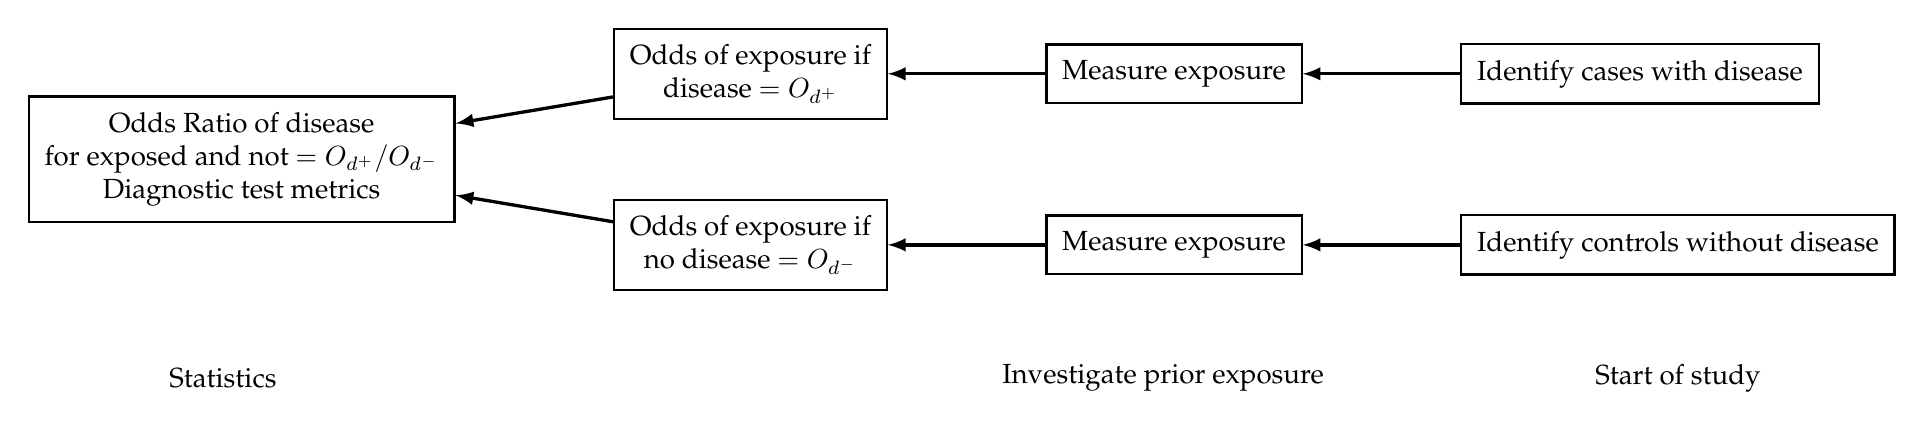
\begin{tikzpicture}[boot/.style={draw,thick,align=center, inner sep=2mm}]

\node[boot=20] (STAT) {Odds Ratio of disease \\  for exposed and not $ = O_{d^+}/ O_{d^-}$\\ Diagnostic test metrics };
\node[above right=0.5cm and 2cm of STAT.east,boot=20] (OD) {Odds of exposure if \\ disease $=O_{d^+}$};
\node[below right=0.5cm and 2cm of STAT.east,boot=20] (OND) {Odds of exposure if \\ no disease $=O_{d^-}$};
\node[right=2cm of OD,boot=20] (ME1) {Measure exposure};
\node[right=2cm of OND, boot=20] (ME2) {Measure exposure};
\node[right=2cm of ME1,boot=20, anchor=west] (ICa) {Identify cases with disease};
\node[right=2cm of ME2, boot=20, anchor=west] (ICo) {Identify controls without disease};



\node[below=1cm of ICo,align=center] (SS) {Start of study};
\node[left=3.2cm of SS, align=center] (IPE) {Investigate prior exposure};
\node[left=16.5cm of SS,align=center] (STATD) {Statistics};

\draw (ICa) edge[standard edge] (ME1)
(ICo) edge[standard edge] (ME2)
(ME1) edge[standard edge] (OD)
(ME2) edge[standard edge] (OND)
(OD) edge[standard edge] (STAT)
(OND) edge[standard edge] (STAT);
\end{tikzpicture}}
\end{center}
}

\frame{
	\frametitle{Measuring outcomes}
	\begin{itemize}
\item Cohort study: Relative Risk
\item Case-control study:  Odds Ratio 
\end{itemize}
\begin{center}
\begin{longtable}{r c c}
\toprule
Risk factor & Cases with disease & Controls without disease \\
\toprule 
Exposed & a & b \\
\midrule
Not exposed & c & d \\
\bottomrule
\caption{$OR = \frac{a/c}{b/d}$}
\end{longtable}
\end{center}

\vspace{-.5cm}
\begin{center}
\begin{longtable}{r c c c}
\toprule
Developed the disease & Exposed & Not exposed & Total \\
\toprule 
Yes & a & b &a+b \\
\midrule
No & c & d &c+d \\
\bottomrule
\caption{$RR = \frac{a/(a+c)}{b/(b+d}$}
\end{longtable}
\end{center}

}
	
\section{What is a biobank?}
\frame{
	\frametitle{What is a biobank}
	\begin{block}{A new kind of large cohorts}
\textbf{Biobanks:} large biomedical databases containing data on participants from traditional questionnaires, in addition to biological samples, for instance to help evaluate the association between genetic variation, environmental exposures for risk of disease.
	\end{block}
\begin{figure}
\centering

\includegraphics[width=.8\textwidth]{Immagini/Biobank.png} 
\end{figure}
	
}



\section{Small group activity: case-control and cohort designs}
\subsection{Exercise (30 minutes)}
\frame{
\frametitle{Scenario}
\begin{itemize}[<+->]
\item Pancreatic cancer: 10th most common cancer, with the lowest survival.
\item Early diagnosis is crucial to improve survival outcomes.
\item Some data provide preliminary support for use of imaging methods (endoscopic ultrasound and MRI) if patients screened are \textbf{at increased risk} of pancreatic cancer. Therefore an accurate, non-invasive way to identify people at sufficiently risk could enable the development of pancreatic cancer screening. 
\item There have  been investigations on the utility of a variety of \textbf{biomarkers} to identify those at sufficiently increased risk of pancreatic cancer to justify screening using imaging.
\item Barts Cancer Institute is the Pancreatic Cancer Research Fund Tissue Bank - set up in 2016, it has collected:
\begin{itemize}
\item Blood samples from 2,200 consenting patients who underwent biopsies or surgery for pancreatic diseases, including pancreatic cancers (also urine, saliva and tissue samples);
\item Large numbers of healthy control blood (also urine and saliva).
\end{itemize}
\end{itemize}

}
\frame{
\frametitle{Question 1}
\begin{block}{Which study design is appropriate?}
How would you design a study to investigate whether or not a proposed biomarker (or a combined panel of biomarkers) is an effective tool for identifying those at high risk of pancreatic cancer, in order to enable early detection of pancreatic cancer?
\end{block}

}


\frame{
\frametitle{Question 2}
\begin{block}{How measure?}
What summary measure of risk associated with the biomarker could you use for each study?
\end{block}
}


\frame{
\frametitle{Main research question}
\begin{block}{We've got funding!}
Assume that Cancer Research UK is going to fund \textbf{two different studies} to investigate \textbf{whether your research group’s biomarker panel can help stratify risk of pancreatic cancer}, and enable early detection that might lead to improvements in public health outcomes. One will be a \textbf{case-control study}, that will report its results within 3 years and the other will be a \textbf{cohort study} which will report its results within 13 years.
\end{block}
}
\subsection{Presentation (30 minutes)}


\section{Review of STAT 1-3 MCQs}
\frame{
	\frametitle{Review of MCQ from STAT1 - STAT3}
	\begin{block}{Join the menti quiz:}
	Join the poll at the link
	\begin{center}
		\url{https://www.menti.com/zc2nq3h3mq}
	\end{center}
	Or go to \url{https://www.menti.com} and use the code \textbf{2106 7080}.
	\end{block}
	
	\begin{figure}
		\centering
		
\includegraphics[height=0.5\paperheight]{Immagini/mentimeter_qr_code}
	\end{figure}
}




{
\setbeamercolor{background canvas}{bg=}
\includepdf[pages=2]{QM-presentation-template.pdf}
}





\end{document}
